
\subsection{Data Collection}
The Nyke Shoe Company collected data on gender, shoe size, and height for the purpose of determining whether or not they can change their business model to include only one size of shoes—regardless of height or gender of the wearer. See Table \ref{fig:MainData} for data collected.

The design and implementation of the data collection is not known\footnote{Contact Nyke Shoe Company for details about data collection.}; there may be bias supporting their business model change. Several important variables related to shoe size were not supplied, including: age, ethnicity, and income. In addition, the sample size of 35 is not large enough to base large-scale business changes on.

\subsection{Analysis}
The sample size of 35 is sufficient to practically perform the following statistical analysis:
\begin{enumerate}
    \item Synthesize hypotheses
    \item Test normality of data
    \item Identify relationships between data
    \item Accept or reject hypotheses based on statistical tests
\end{enumerate}
\par

\subsubsection{Synthesize Hypotheses}
To synthesize the null and alternative hypotheses, the business objective was first identified: Should Nyke Shoe Company disregard height or gender for changing their business model to include only one size of shoes? In other words, are height and gender significantly associated with shoe size?

To answer the business objective, null and alternative hypotheses were formed for the relationship between height and shoe size:
\begin{align*}
H_0 &:& \text{There is a significant relationship between height and shoe size.}\\
H_A &:& \text{There is not a significant relationship between height and shoe size.}
\end{align*}
Null and alternative hypotheses were also formed for the relationship between gender and shoe size:
\begin{align*}
H_0&:&\text{There is not a statistically significant relationship between gender and shoe size.} \\
H_A&:&\text{There is a statistically significant relationship between gender and shoe size.}
\end{align*}

\subsubsection{Test Normality}
The normality of the data was tested to verify the normality assumption for statistical tests. Microsoft Excel was used to generate the following descriptive statistics values to describe all sampled shoe sizes, Male shoe sizes, and Female shoe sizes.

\begin{longtable}{|c|c|c|c|}
\caption{\label{tab:DescriptiveStats}Descriptive statistics table.}\\
\hline
\cellcolor{gray} & All & Male & Female \\
\hline
Mean & 9.142857 & 11.29412 & 7.111111 \\
Standard Error & 0.43655 & 0.437361 & 0.266776 \\
Median & 9 & 11 & 7 \\
Mode & 7 & 11 & 7.5 \\
Standard Deviation & 2.582667 & 1.803285 & 1.131833 \\
Sample Variance & 6.670168 & 3.251838 & 1.281046 \\
Kurtosis & -1.08309 & 0.687533 & 1.830705 \\
Skewness & 0.366603 & -0.45407 & 0.854222 \\
Range & 9 & 7 & 5 \\
Minimum & 5 & 7 & 5 \\
Maximum & 14 & 14 & 10 \\
Sum & 320 & 192 & 128 \\
Count & 35 & 17 & 18 \\
\hline
\end{longtable}
\par
Using the values generated in table \cref{tab:DescriptiveStats}, Pearson's chi-squared statistic was calculated. First, expected frequencies were calculated based on the normal distribution for each value based on Standard Error and Mean. The chi-squared statistic was then computed based on the differences from the expected frequencies


\subsubsection{Identify Relationships}
Linear regression on the data provided by Nyke Shoe Company was performed in Microsoft Excel; this was done to identify a potential correlation between height and shoe size\footnote{See Table \ref{tab:LinearRegression} for full linear regression output.}. The following information was generated from performing linear regression:
\begin{align*}
    &\hat{y} = 0.554x + -29.057 \\
    &r = 0.864\\
    &r^2 = 0.747\\
    &\sigma_{\overline{x}} = 1.318 \\
\end{align*}
Because the absolute value the coefficient of determination {$r^2$} is above {$0.5$}, the linear correlation between height and shoe size is relatively strong. Notice the close match between the pattern of data points and the regression line in the following graph:
\par
\begin{minipage}{\linewidth}
    \centering
    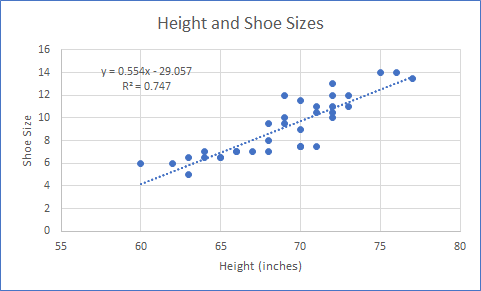
\includegraphics{graphics/HeightAndShoeSizesRegressionLine.png}
    \captionof{figure}{Regression line plotted with data points.}
    \label{fig:RegressionLine}
\end{minipage}
\par
\vspace{5cm}
Because the gender variable is categorical, the relationship between gender and shoe size was identified using the independent samples t-test instead of linear regression.


\subsubsection{Test Hypotheses}